\chapter{Human-guided iterative training \protect\\ of dynamic motions}
Resembles learning by demonstration,

\section{Prior Work: Iterative Training Of Dynamic Skills Inspired By Human Coaching Techniques}

In our prior work \cite{Ha:2014:ITD},
we introduce an intuitive and interactive framework for developing 
dynamic controllers inspired by how humans learn dynamic motor
skills through progressive process of coaching and practices. 
The user only needs to provide a primitive initial controller and
high-level, human-readable instructions as if
she is coaching a human trainee, while the character has the ability
to interpret the abstract instructions, accumulate the knowledge from
the coach, and improve its skill iteratively. We introduce ``control
rigs'' as an intermediate layer of control module to facilitate the
mapping between high-level instructions and low-level control
variables. Control rigs also utilize the human coach's knowledge to
reduce the search space for control optimization. In addition, we
develop a new sampling-based optimization method, Covariance Matrix
Adaptation with Classification (CMA-C), to efficiently compute control
rig parameters. Based on the observation of human ability to ``learn
from failure'', CMA-C utilizes the failed simulation trials to
approximate an infeasible region in the space of control rig
parameters, resulting a faster convergence for the CMA
optimization. 
Without using motion trajectories, or tuning any parameters,
We demonstrate the design process of complex dynamic
controllers using our framework, including precision jumps, turnaround
jumps, monkey vaults, drop-and-rolls, and wall-backflips 
(\figref{training1_teaser}).


\begin{figure}[htbp]
\center
  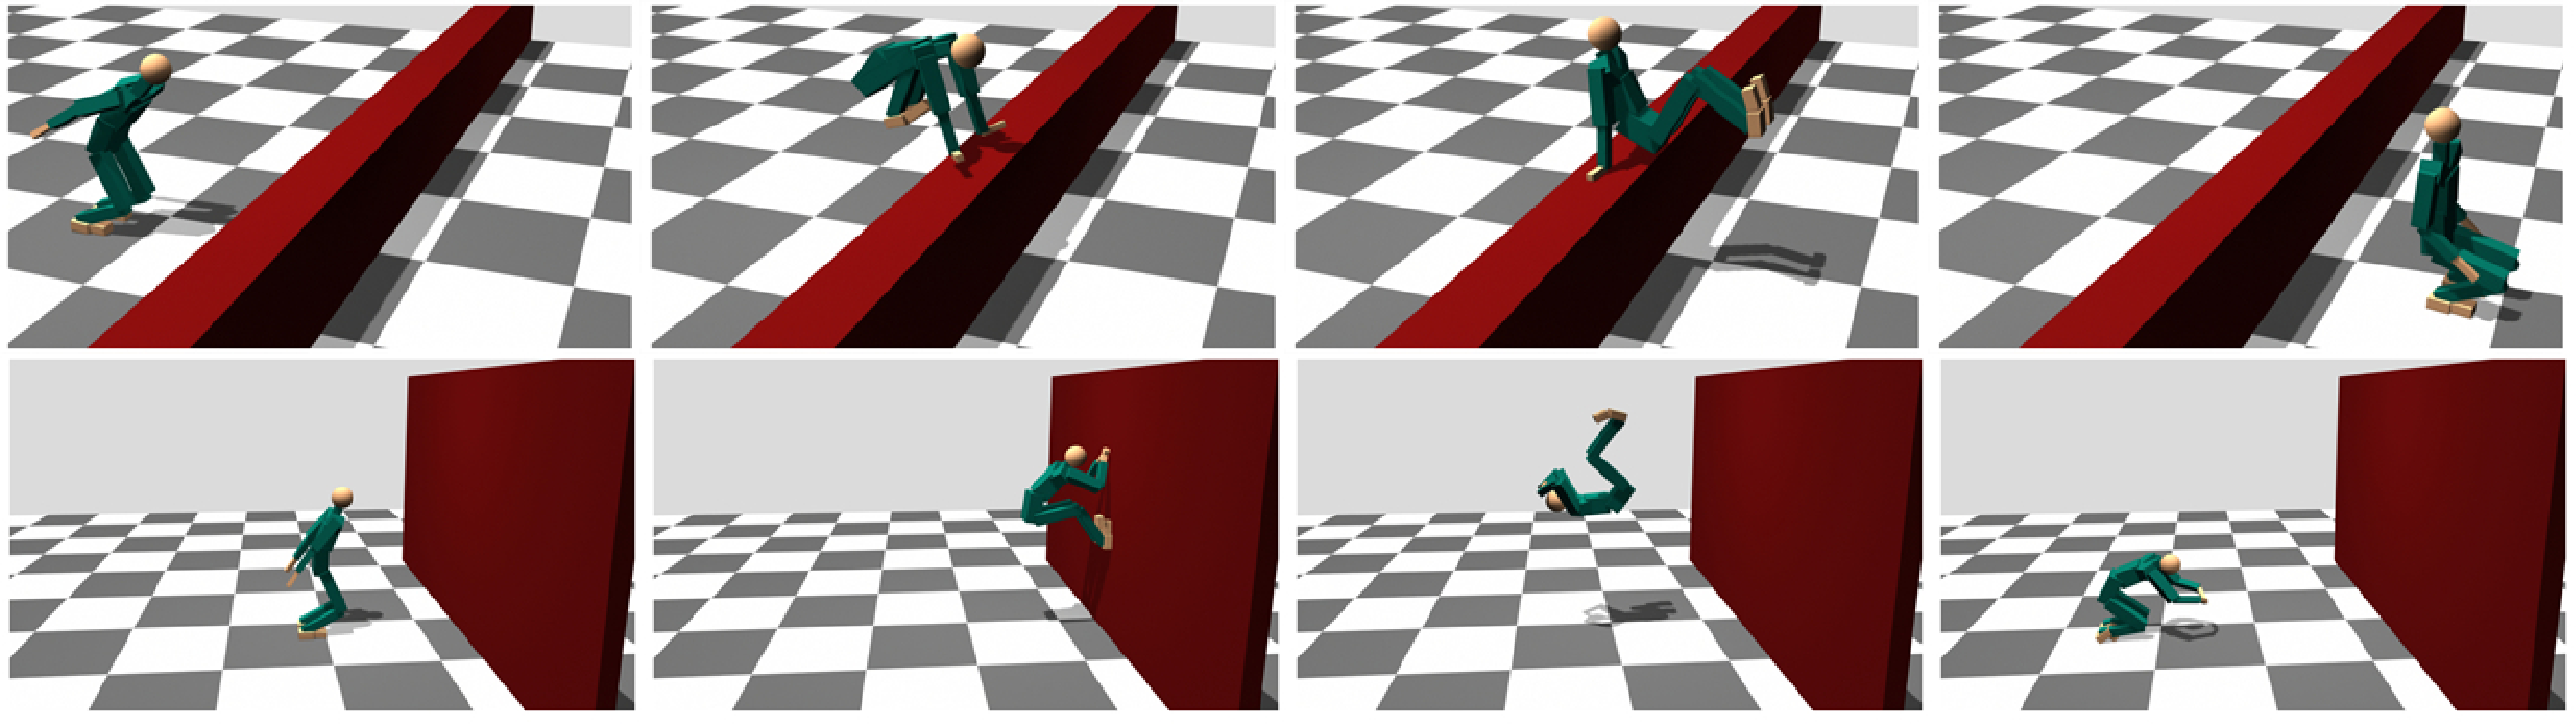
\includegraphics[width=\linewidth]{images/training1_teaser}
  \caption{Monkey vault (Top) and wall-backflip (Bottom).}
 \label{fig:training1_teaser}
\end{figure}


\section{Iterative Training Of Dynamic Skills for Humanoid Robots}


\subsection{Problem Description}

\subsection{Related Work}

Learning from demonstration (LfD), also known as programming by demonstration,
has been an attractive paradigm for training motor skills to robots.
In this paradigm, a set of examples are provided by human teachers,
and an optimal policy is generated from such examples.
Since the early work of Kuniyoshi \etal \cite{kuniyoshi:1989:TBS},
it has been proven to be effective for training motor skills in
numerous task domains, including object manipulation 
\cite{Atkeson:1997:RLD,Calinon:2007:LRG,Ueda:2010:MNH},
navigation \cite{Konidaris:2011:RLD}, 
full-body motion generation \cite{Kulic:2011:ILF}, and so on.
To increase the robustness, the learned motor skills are further 
generalized using machine learning techniques,
such as gausian mixture model \cite{Calinon:2007:LRG} or
motion primitives \cite{Pastor:2009:LGM}.
However, dynamic motor skills of humanoids have
not been fully examined yet, except the only few works on the
locomotion \cite{Nakanishi:2004:LDA}, which is our target domain
in this proposal.

\subsection{System Overview}
